\section{Introduction to Redundant Complexification}
In the hallowed realms of engineering academia, it is a well-established fact that no concept is too simple to be made complex. This paper serves as a beacon of enlightenment, guiding the uninitiated through the sacred art of making straightforward ideas bewilderingly intricate.

\subsection{Theoretical Foundations of Over-Engineering}
This subsection embarks upon a verbose journey into the heart of engineering complexity, elucidating the fundamental principles that govern the unnecessary complication of otherwise uncomplicated matters.

\subsubsection{Quantifying the Unquantifiable}
With rigorous hand-waving and the strategic application of buzzwords, we delve into the mathematical morass of engineering hyperbole. Here, we introduce the "Complexity Coefficient," \( C = \frac{n}{s} \), where \( n \) represents the number of needless components, and \( s \) the simplicity of the initial problem \cite{conferencepaper}.

Figure \ref{fig:overengineered_paperclip} shows a schematic diagram of an over engineered paperclip which serves as an example to the time-honored engineering tradition of fixing what isn't broken.

\begin{figure}[H]
\centering
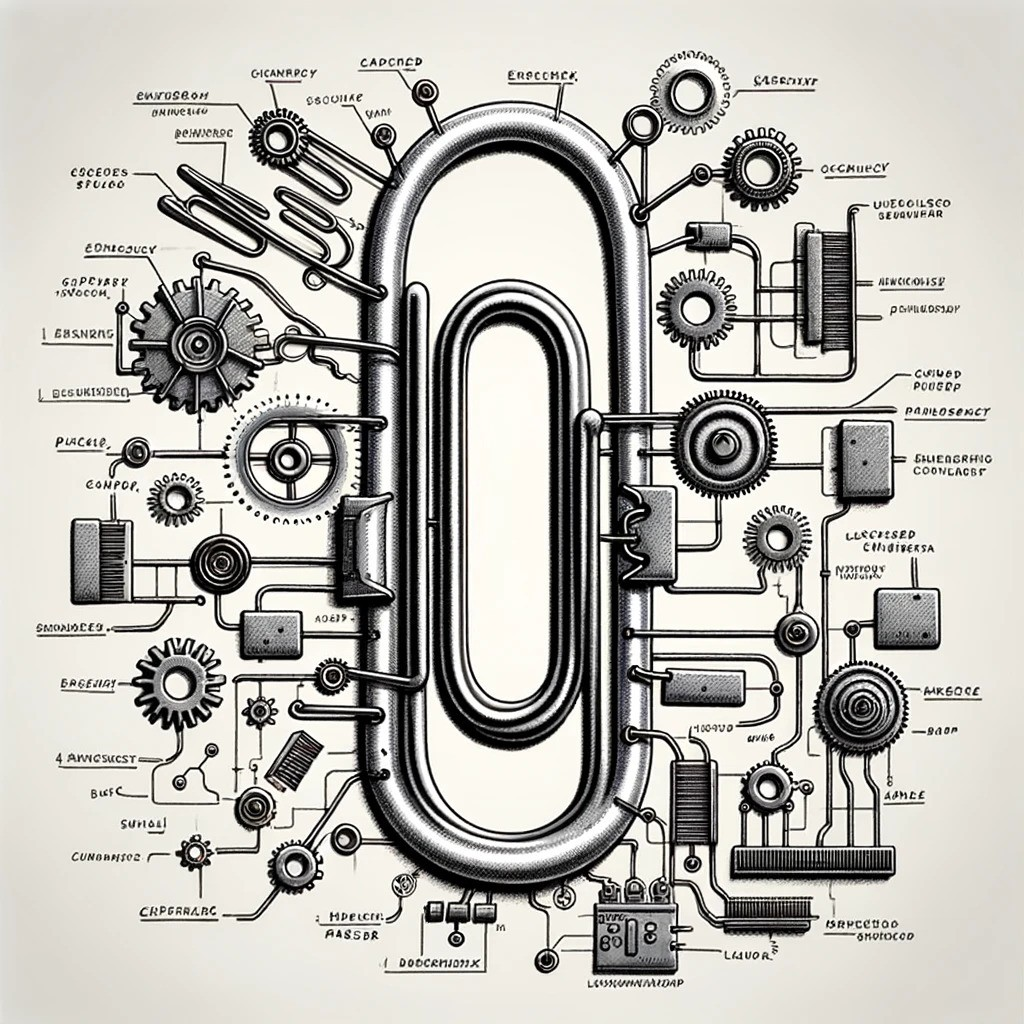
\includegraphics[width=0.5\textwidth]{Images/engineering_overcomplication.jpg}
\caption{A Schematic Diagram of an Over-Engineered Paperclip}
\label{fig:overengineered_paperclip}
\end{figure}

This is a great place to throw a random citation \cite{author2020} to make it look like I've read the literature.